\documentclass{ProjectReport}
\Protitle{\large{SOME CONTRIBUTION TO \LaTeX TO FACILITATE DOCUMENT FORMATTING IN A TECHNICAL INSTITUTE}}
\MemberA{Shilpa S. Mahadik}	\RegA{T-08-38}
\MemberB{Sadaf H. Desai}		\RegB{T-08-07}
\MemberC{Sayali S. Kalyani}		\RegC{T-08-06}
\MemberD{Bhagyashree V. Chavan}	\RegD{T-08-36}
\Guidename{Mr. S. V. Jadhav}
\begin{document}
\frontmatter
\pagenumbering{roman}
\makepreliminarypages

\addcontentsline{toc}{chapter}{Abstract}
\chapter*{Abstract}
\LaTeX is a document preparation system that enables the document writer to concentrate on the contents without bothering much about the formatting. The basic \LaTeX software system is available free of charge.

The aim of the project is to generate class or style files in \LaTeX, which can be used by students/faculty/staff of Finolex Academy of Management and Technology to format generally, used documents such as, project reports, notices, handouts, internal notes, etc. The classes in \LaTeX provide automation to improve consistency, productivity, and accuracy in creating and maintaining documents, thereby avoiding the inefficiencies of word processors.

\tableofcontents
\listoffigures

\mainmatter
\chapter{Project Overview}
\setcounter{page}{1}
\thispagestyle{empty}
\LaTeX purpose is to simplify \TeX typesetting. \LaTeX has the provision of creating user-defined style and class files.

The project - Some contribution to \LaTeX to facilitate document formatting in a technical institute -attempts to create class files for project reports and notices as per technical specifications. 

A standard project report includes key points - title page, certificate page, abstract, contents, references, appendix and acknowledgements. The title page in a standard project report has key fields - project title, degree or course, college name, department name, name and registration number of the students involved in the project, name of the project guide and logo of college. In addition to these fields, the certificate page in a standard project report includes the university to which the college is affiliated. 

Care has been taken that these above mentioned fields in project report will be typeset as per the standards of the college Finolex Academy of Management and Technology. These fields are not limited to their default values, but a provision has been made for users outside this college to use these class files by changing default parameters for their project reports.

For this purpose,  the project facilitates the typesetting by making default specifications for the page alignment, line spacing, font sizes, styles, headers, footers, figures, equations, etc.
Thus the project helps in best possible way to reduce the user efforts in documentation, by making it more handy and less time consuming.

Pre-requisites for project are - at a minimum, you'll need a \TeX distribution, a good text editor and a PDF viewer.

\chapter{Introduction and Motivation}
\thispagestyle{empty}
The generally used documents such as project reports, notices, internal notes etc. in any technical institute are expected to be submitted in a standard specified format. The commonly used editing tools for this purpose are Microsoft Word, notepad, wordpad, etc. Taking into consideration various formatting constraints namely alignment, font styles, paragraphs, sections, subsections, etc. becomes a bit tedious using MS Word or other tools. Also maintaining the subscripts and superscripts to obtain the various mathematical equations becomes difficult and time consuming.

To overcome this drawback we have \LaTeX, a documentation preparation system that enables the document writer to concentrate on the contents of their text, without bothering too much about the formatting of it. 

\section{An Introduction to \LaTeX}
\LaTeX is a document preparation system for high-quality typesetting. It is most often used for medium-to-large technical or scientific documents but it can be used for almost any form of publishing.

\LaTeX is not a word processor. \LaTeX is based on the idea that authors should be able to focus on the content of what they are writing without being distracted by its visual presentation. In preparing a \LaTeX document, the author specifies the logical structure and lets the \LaTeX system worry about the presentation of these structures. It therefore encourages the separation of layout from content while still allowing manual typesetting adjustments where needed.

\LaTeX is based on Donald E. Knuth's \TeX typesetting language or certain extensions. \LaTeX was first developed in 1985 by Leslie Lamport.

\section{Why \LaTeX?}
What you see is what you get (WYSIWYG) programs make it easy to put text wherever you want in whatever size and style of type you want, i.e., WYSIWYG programs offer visual design. The visual design is fine for short, simple documents like letters and memos. The visual design is not good for more complex documents such as scientific papers. For this purpose, we use \LaTeX that offers logical design.

\LaTeX is intended to provide a high-level language that accesses the power of \TeX. \LaTeX comprises a collection of \TeX macros and a program to process \LaTeX documents. Because the \TeX formatting commands are very low-level, it is usually much simpler for end-users to use \LaTeX .
As \LaTeX is distributed under the terms of the \LaTeX Project Public License (LPPL), \LaTeX is free software.

\section{Required Parts of \LaTeX input file}
A few commands must appear in every \LaTeX input file in a certain order. They are:
\begin{verbatim}
\documentclass{classname}
\begin{document}
\end{document}
\end{verbatim}
The documentstyle has a required argument stylename to select an overall type-setting style for the document; the one normally used is article (there are also book, report, letter, and memo). It also has an optional argument to select 11pt or 12pt normal type size (10pt is the default size). The actual text of user document and associated commands go between the begin and end commands.

\section{Customizing \LaTeX}
There are situations where \LaTeX does not provide a command or environment that matches user needs, or the output produced by some existing command may not meet user requirements.To add your own commands, use
\begin{verbatim}
\newcommand{name}[num]{definition}
\end{verbatim}
The command requires two arguments: the name of the command you want to create, and the definition of the command. The num argument in square brackets is optional.
\subsection{Creation of style file}
Typically, a style sheet is specified at the beginning of document. This style sheet applies to the entire document. To create your own style file, at the very beginning of the text document just write,
\begin{verbatim}
\ProvidesPackage{mypack}
\end{verbatim}
where mypack is the name of package. Write whatever you want in it using all the \LaTeX commands you know. The style file should have the same name as that of the
package name. Save this style file with extension .sty. Now, it is necessary to import this style file in your \TeX document which can be done using following command.
\begin{verbatim}
\usepackage{mypack}
\end{verbatim}
where mypack is the style file you have created earlier.

\subsection{Creation of class file}
Create a simple file called myclass.cls and open it with any text editor, at the very beginning of the document just write
\begin{verbatim}
\NeedsTeXFormat{LaTeX2e}
\ProvidesClass{<class-name>}[<date><other information>]
\end{verbatim}
Write whatever you want in it using all the \LaTeX commands you know. Import your new class with the known command
\begin{verbatim}
\documentclass{myclass}
\end{verbatim}
The file myclass.sty and the \LaTeX source you are compiling must be in the same directory.

\section{Motivation}
The existing word processors have several limitations which can be overcome by \LaTeX. The main advantages of \LaTeX over normal word processors are the following:
\begin{itemize}
\item Professionally crafted layouts are available, which make a document really look as if ``printed''.
\item The typesetting of mathematical formulae is supported in a convenient way.
\item Users only need to learn a few easy-to-understand commands that specify the logical structure of a document. They almost never need to tinker with the actual layout of the document.
\item Even complex structures such as footnotes, references, table of contents, and bibliographies can be generated easily.
\item Free add-on packages exist for many typographical tasks not directly supported by basic \LaTeX. For example, packages are available to include PostScript graphics or to typeset bibliographies conforming to exact standards. 
\item \LaTeX encourages authors to write well-structured texts by specifying structure.
\end{itemize}

\chapter{Problem Statement}
\thispagestyle{empty}
The proposed system attempts to use \LaTeX to make documentation of generally used documents like project thesis, reports, notices, etc. in the technical institutes a bit easier.
The proposed system will provide class or style files for a technical institute to write
\begin{enumerate}
\item notices
\item project reports
\end{enumerate}
The user simply needs to include the package name in his file and use the commands defined in the package to format his documents. Thus, the proposed system will reduce the efforts of the user in formatting the documents.

\chapter{Implementation Details}
\thispagestyle{empty}
\section{List of packages}
The list of packages required to implement this project are:
\begin{enumerate}
\item graphicx \\
This package is an extension of the standard graphics bundle and provides a way to include repeated postscript graphics (ps, eps) only once in a postscript document. This provides a way to get smaller postscript documents when having, for instance, a logo on every page. This package only works when post-processed with dvips.
\item epstopdf \\
The package adds support for EPS files in the graphicx package when running under PDFTeX. If an EPS graphic is detected, the package spawns a process to convert the EPS to PDF, using the script epstopdf. This of course requires that shell escape is enabled for the PDFTeX run.
\item ifthen \\
Conditional commands in \LaTeX documents \\
The package's basic command is \begin{verbatim} \ifthenelse \end{verbatim} which can use a wide array of tests. Package also provides a simple loop command \begin{verbatim} \whiledo \end{verbatim}
\item xifthen \\
Extended conditional commands \\
This package extends the ifthen package by implementing new commands to go within the first argument of \begin{verbatim} \ifthenelse \end{verbatim} to test whether a string is void or not, if a command is defined or equivalent to another. The package also offers the possibility to make use of complex expressions, together with the ability of defining new commands to handle complex tests.
\item changepage \\
Margin adjustment and detection of odd/even pages \\
The package provides commands to change the page layout in the middle of a document, and to robustly check for typesetting on odd or even pages. Instructions for use are at the end of the file. The package is an extraction of code from the memoir class, whose user interface it shares. It is intended this package will eventually replace the chngpage package, which is distributed with the package.
\item geometry \\
Flexible and complete interface to document dimensions \\
The package provides an easy and flexible user interface to customize page layout, implementing auto-centering and auto-balancing mechanisms so that the users have only to give the least description for the page layout. 
\item fontenc \\
Standard package for selecting font encodings \\
The package allows the user to select font encodings, and for each encoding provides an interface to font-encoding-specific commands for each font. Its most powerful effect is to enable hyphenation to operate on texts containing any character in the font.
\item mathptmx \\
This package defines Adobe Times Roman (or equivalent) as default text font, and provides maths support using glyphs from the Symbol, Chancery and Computer Modern fonts together with letters, etc., from Times Roman. It supersedes both the original times and the mathptm packages.
\item fancyhdr \\
Creating headers and footers in \LaTeX can be done by using the package ``fancyhdr''.  First of all, you need to tell \LaTeX to use the package:
\begin{verbatim}
\usepackage{fancyhdr}
\end{verbatim}
and change the style from plain to fancy:
\begin{verbatim}
\pagestyle{fancy}
\end{verbatim}
You will now get the default fancy pagestyle which adds a line at the top of every page, except for some exceptions (title-page, abstract, new chapter in report).
Even though fancyhdr has a default page style, you are free to define headers/footers yourself.
\item caption \\
Customising captions in floating environments \\
The caption package provides many ways to customise the captions in floating environments like figure and table, and cooperates with many other packages. Facilities include rotating captions, sideways captions, and continued captions (for tables or figures that come in several parts).
\item appendix \\
Extra control of appendices \\
The appendix package provides various ways of formatting the titles of appendices. Also (sub)appendices environments are provided that can be used, for example, for per chapter/section appendices.
\item beamer \\
A \LaTeX class for producing presentations and slides \\
The beamer class can be used for producing slides. It does not need any external programs and can directly produce a presentation using pdflatex. Beamer uses pgf for pdf/ps independent graphics. Frames are created using \begin{verbatim} \frame{...} \end{verbatim} Beamer supports bibliographies, appendices and transitions. Short versions of title, authors, institute can also be specified as optional parameters. \begin{verbatim} \plainframe{} \end{verbatim} allows a picture, for example, to fill the whole frame. Support figure and table environments, transparency effects, transduration command, animation commands, pauses environment.
\item hyperref \\
Extensive support for hypertext in \LaTeX \\
The hyperref package is used to handle cross-referencing commands in \LaTeX to produce hypertext links in the document. The package is distributed with the backref and nameref packages, which make use of the facilities of hyperref. The package depends on the author's kvoptions, ltxcmds and refcount packages. 
\end{enumerate}

\section{CollegeNotice.cls}
\subsection{Using the class CollegeNotice}
To use the CollegeNotice class, make sure that the CollegeNotice.cls file is on your TEXINPUTS search path and use the following command at the start of your input file:
\begin{verbatim}
\documentclass{ CollegeNotice}
\end{verbatim}
\subsection{What the CollegeNotice class does}
The CollegeNotice class provides users of Finolex Academy of Management and Technology(FAMT) to prepare a notice according to standard norms. \\
The key features of the class are - By default this class uses FAMT as default college and Information Technology as default department, which can be changed as per user requirements. 

\textbf{Default values for the commands are:} \\
College - Finolex Academy of Management and Technology \\
Department - Information Technology \\
Issuedate - \LaTeX takes current date from the system \\
Desigantion - Head of Department

\textbf{Mandatory values user needs to provide are:} \\
Subject of notice \\
Content of notice

\textbf{To overwrite default values commands to be used are:}
\begin{verbatim}
\College		Specify the name of the college, if it is other than FAMT
\Department	Specify the name of the department, if it is other than IT
\Issuedate	The date when the notice is to be issued
\Name		The name of the person issuing the notice
\Designation	The name of the person issuing the notice
\end{verbatim}

\section{ProjectReport.cls}
\subsection{Using the class ProjectReport}
To use the ProjectReport class, make sure that the ProjectReport.cls file is on your TEXINPUTS search path and use the following command at the start of your input file:
\begin{verbatim}
\documentclass{ProjectReport}
\end{verbatim}
\subsection{What the ProjectReport class does}
The ProjectReport class is a modified version of the standard \LaTeX REPORT class that is accepted for use with Finolex Academy of Management and Technology (FAMT) dissertations theses. The ProjectReport class allows users to concentrate on the content of report instead of formatting.

\textbf{The key features of the class are:}
\begin{enumerate}
\item The title page and certificate page is designed to fulfill the specifications of FAMT institute.
\item Margins are 1.3 inches from the left, 1.1 inches from right, 1.4 inches from top and 1.1 inches from bottom.
\item Uses 12 point by default.
\item Page numbers are in the center at the bottom for all pages.
\item Complete, correct front matter for ProjectReport can be generated.  
\end{enumerate}

\textbf{Default values for commands are:} \\
College -Finolex Academy of Management and Technology \\
Department - Information Technology \\
University- Mumbai University \\
Month - April \\
Degree - Bachelor of Engineering

\textbf{Mandatory values user needs to provide are:} \\
Name of students \\
Registration number of students \\
Name of Guide \\
Title of Project Report

\textbf{To overwrite default values, commands to be used are:} 
\begin{verbatim}
\College
\Department
\University
\Degree
\monthnum
\Year
\end{verbatim}

\textbf{Layout constraints:}
\begin{enumerate}
\item Margins - Using geometry package, margins are set to 1.3 inches from the left, 1.1 inches from right, 1.4 inches from top and 1.1 inches from bottom.
\item Headers and Footers - Using fancyhdr package, page numbers are set in the center at the bottom for all pages and section name in header at the right corner.
\item Fonts - Using fontenc, mathptmx package, the default font size is set to 12, font family is set to Times New Roman.
\end{enumerate}

\textbf{Front matter:} \\
The title page, certificate page, abstract, table of contents, lists of figures MUST be put inside the "frontmatter" environment, which ensures that page-numbering is handled properly. 

\textbf{College Logo and other Figures:} \\
The College Logo is provided in eps format so that it cannot be edited. To include Logo.eps into the Project Report the package eps2pdf is used. \\
The figures related to project should be included in figure environment to ensure that numbering is handled properly.

\chapter{Technologies Used}
\thispagestyle{empty}
The recommended \TeX distributions are:
\begin{itemize}
\item \TeX Live is a major \TeX distribution for Unix/Linux, Mac OS and Windows.
\item MiKTeX  is a Windows-specific distribution.
\item MacTeX  is a Mac OS-specific distribution based on \TeX Live.
\end{itemize}
In project, MikTeX 2.9 has been used.

\section{MikTeX - An Introduction}
MiKTeX (pronounced mick-tech) is a typesetting system for Microsoft Windows that is developed by Christian Schenk. MiKTeX provides the tools necessary to prepare documents using the \TeX/\LaTeX markup language. 
The current version of MiKTeX is 2.9. Since version 2.7, MiKTeX has compatibility with Windows 7. MiKTeX is currently being ported to GNU/Linux, with a beta version being available for testing.

\section{Features of MikTeX}
\begin{enumerate}
\item Easy to install \\
It is very easy to install MiKTeX. The MiKTeX Setup Wizard guides you through the installation process. You don't have to be a computer expert. 
\item Complete \\
A complete set of additions (programs, styles, fonts, \ldots) are available to help you typeset your documents.
\item Integrated package management \\
MiKTeX's integrated package manager installs missing components from the Internet, if required.

For example, the \LaTeX directive
\begin{verbatim}
\usepackage{memoir}
\end{verbatim}
would trigger the installer, if the memoir package is not already installed.

This unique feature allows you to keep your computer clutter-free: only install packages you actually need.
\item Network friendly \\
MiKTeX can be run directly from a shared and read-only network directory
\item Enhanced \TeX compiler capabilities
\item Always up-to-date \\
The MiKTeX Update Wizard helps you to keep your MiKTeX system up-to-date by installing the latest package updates.
\item Fast previewer \\
The \TeX output viewer Yap allows for an optimized edit-compile-view cycle (if the \TeX authoring system in use supports source specials).
\item Well maintained \\
The MiKTeX package repository is updated regularly
\item Open source \\
 MiKTeX is open source. You are welcome to redistribute MiKTeX under certain conditions. 
\end{enumerate}

\section{Components of MikTeX}
The MiKTeX distribution consists of the following components:
\begin{itemize}
\item \TeX, METAFONT, TeXware, METAFONTware, Computer Modern Fonts-the base \TeX system
\item pdfTeX, XeTeX, Omega, NTS-various \TeX derivatives
\item MetaPost-a METAFONT derivative for the creation of PostScript figures
\item Dvipdfm-converts \TeX output into PDF documents
\item macro packages-almost all free \TeX macro packages
\item fonts-almost all free fonts
\item TeXify-a \TeX compiler driver
\item MiKTeX Options-assists in configuring MiKTeX
\item MiKTeX Update Wizard-assists in keeping the MiKTeX system up-to-date
\item lots of utilities tools for the creation of bibliographies \& indexes, PostScript utilities
\end{itemize}

\section{Utilities in MikTeX}
A few utilities required in MiKTex packaging are:
\begin{enumerate}
\item cabextract \\
cabextract is used intnernally (by MPC) to extract files from cabinet files. It is a part of the Cygwin distribution for Windows.
\item lzma \\
lzma is used intnernally (by MPC) to extract files from .tar.lzma files. It is a part of the Cygwin distribution for Windows.
\item md5walk \\
MD5Walk is used to calculate the fingerprint of a package. The source code of MD5Walk can be obtained from the MiKTeX project page.
\item mpc \\
The MiKTeX Package Creator (MPC) is used to maintain the contents of a custom package repository. The source code of MPC can be obtained from the MiKTeX project page.
\item rsync \\
rsync is used to initialize the custom package repository. It is a part of the Cygwin distribution for Windows.
\item tar \\
tar is used internally (by MPC) to create package archive files. It is a part of the Cygwin distribution for Windows.
\end{enumerate}
All but MPC and MD5Walk are standard utilities which are available on all platforms (Windows, GNU/Linux, \ldots). The portable source code of mpc and md5walk can be obtained from the MiKTeX project page.

\chapter{Project Timeline}
\thispagestyle{empty}
\begin{figure}[h]
\centering 
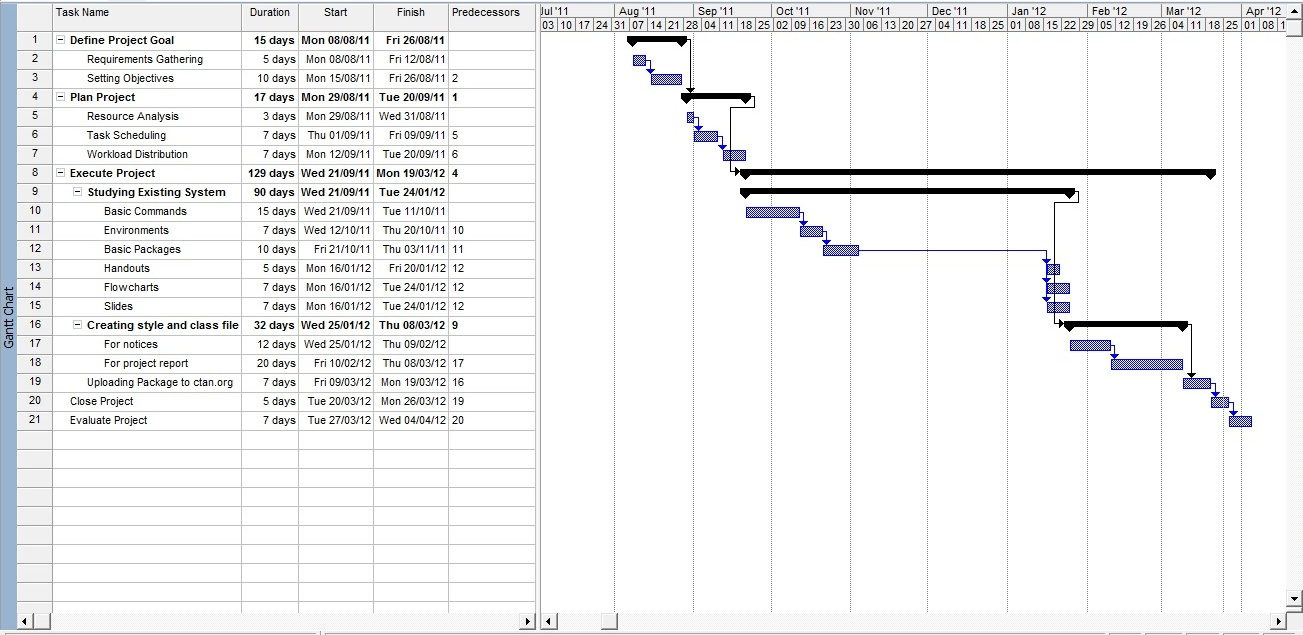
\includegraphics[width=1.10\textwidth]{./Ganttchart}
\caption{Gantt Chart}
\end{figure}

\chapter{Task Distribution}
\thispagestyle{empty}
\begin{figure}[h]
\centering 
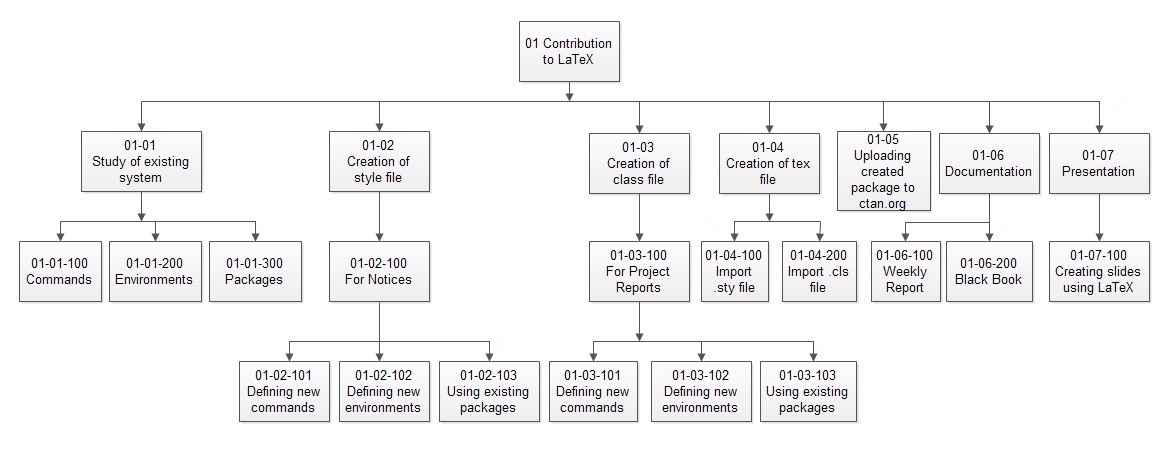
\includegraphics[width=1.10\textwidth]{./WBS}
\caption{Work Breakdown Structure}
\end{figure}

\chapter{Conclusion and Future Work}
\thispagestyle{empty}
\section{Conclusion}
Thus our project ``Some contribution to \LaTeX to facilitate document formatting in technical institute'' concentrates on the documentation of notices, project reports which includes project title page, certificate etc. The standard formatting constraints for these documents are defined in packages developed under this project, which will thus help the user to complete his/her work in stipulated time and making it less tedious.  

\section{Future Work}
In order to make use of class files developed in the project, the basic requirement is that the user must have the sound knowledge of  \LaTeX. So to make it more handy,  user interface can be developed which will take only the required values as input viz;  the content of notice and the packages in the back-end will take care of formatting without the user having to know \LaTeX commands.

\addcontentsline{toc}{chapter}{References}
\chapter*{References}
\begin{enumerate}
\item A document preparation system \LaTeX -Leslie Lamport
\item http://tug.org/tutorials/tugindia/
\item http://www.andy-roberts.net/writing/latex
\item http://miktex.org
\item http://www.ctan.org/
\end{enumerate}

\addcontentsline{toc}{chapter}{Acknowledgements}
\chapter*{Acknowledgements}
The efforts taken in this project would not have been possible without the kind support and help of many individuals. We would like to extend sincere thanks to all of them. \\
We are highly indebted to Mr. S.V. Jadhav for his invaluable guidance and constant supervision as well as for providing necessary support in completing the project. \\
We would like to express gratitude towards Mr. Parag Abhyankar for his encouragement which helped us in completion of this project. \\
We would like to express our special gratitude and thanks to all those user groups and communities who have worked on open source document preparation system \LaTeX and have made available their work for our use. \\
Shilpa Mahadik \\
Sadaf Desai \\
Sayali Kalyani \\
Bhagyashree Chavan

\addcontentsline{toc}{chapter}{Appendix}
\chapter*{Appendix}
It is .tex file of project report.
\begin{verbatim}
\documentclass{ProjectReport}
\Protitle{Title of Project}
\MemberA{Shilpa S. Mahadik}	\RegA{T-08-38}
\MemberB{Sadaf H. Desai}		\RegB{T-08-07}
\MemberC{Sayali S. Kalyani}		\RegC{T-08-06}
\MemberD{Bhagyashree V. Chavan}	\RegD{T-08-36}
\Guidename{Mr. S. V. Jadhav}
\begin{document}
\frontmatter
\makepreliminarypages
\chapter*{Abstract}
\tableofcontents
\listoffigures
\mainmatter
\chapter{Project Overview}
\chapter{Introduction and Motivation}
\chapter{Problem Statement}
\chapter{Implementation Details}
\chapter{Technologies Used}
\chapter{Project Timeline}
\chapter{Task Distribution}
\chapter{Conclusion and Future Work}
\chapter*{References}
\chapter*{Acknowledgements}
\end{document}
\end{verbatim}

\end{document}